\begin{evenBlock}{HOWTO:  Passing (5 min)}

\begin{minipage}[t]{\linewidth}
    \centering
    Review these elements prior to beginning the passing drills so its fresh in their heads.

    %\begin{minipage}{.3\linewidth} % Left column and width
        %\centering
        %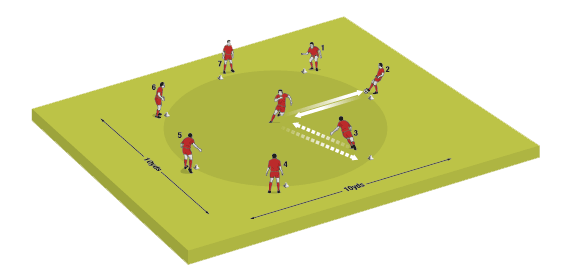
\includegraphics[width=\textwidth]{../img/Trimmed/Clocks1}
    %\end{minipage}
    %\hspace{0.05\linewidth}
    %\begin{minipage}{.6\linewidth} % Left column and width
    
        \textbf{Elements of the Pass:}
    
        \begin{enumerate}
        \setlength{\itemsep}{0pt}
        \setlength{\parskip}{0pt}
        \setlength{\parsep}{0pt}
        \item Ball should start about 1 step in front of the player.
        \item Non-kicking leg should be planted next to the ball with passer's toe pointed at the target.
        \item Ball should be struck in its center,
        \item With the inside portion of the foot.
        \item The kick should follow through.
        \end{enumerate}
        
        \textbf{Elements of the First Touch:}
        \begin{itemize}
        \setlength{\itemsep}{0pt}
        \setlength{\parskip}{0pt}
        \setlength{\parsep}{0pt}
        \item First before the ball is passed be sure you are ready, knees bent and on your toes.
        \item Move your body so the ball is coming directly to you.
        \item Bend your body over the ball as it comes in.
        \item Keep your eye on the ball as it comes into contact with your foot.
        \item Let your foot cushion the ball to slow it down and keep it near your feet.
        \item As your skill develops your first touch can move the ball into the space in which you want (open space or away from the defender).
        \end{itemize}

    %\end{minipage}
\end{minipage}

\end{evenBlock}